\documentclass[12pt]{article}
\usepackage[english]{babel}
\usepackage{natbib}
\usepackage{url}
\usepackage[utf8x]{inputenc}
\usepackage{amsmath}
\usepackage{graphicx}
\graphicspath{{images/}}
\usepackage{parskip}
\usepackage{fancyhdr}
\usepackage{subcaption}
\usepackage{relsize}
\usepackage{vmargin}
\setmarginsrb{3 cm}{2.5 cm}{3 cm}{2.5 cm}{1 cm}{1.5 cm}{1 cm}{1.5 cm}

\title{Statistical Pattern Recognition}								% Title
\author{94131091}								% Author
\date{\today}											% Date

\makeatletter
\let\thetitle\@title
\let\theauthor\@author
\let\thedate\@date
\makeatother

\pagestyle{fancy}
\fancyhf{}
\rhead{\theauthor}
\lhead{\thetitle}
\cfoot{\thepage}

\newcommand\numberthis{\addtocounter{equation}{1}\tag{\theequation}}
\newcommand{\gl}{^{>^{w_1}}_{<_{w_2}}}
\begin{document}

%%%%%%%%%%%%%%%%%%%%%%%%%%%%%%%%%%%%%%%%%%%%%%%%%%%%%%%%%%%%%%%%%%%%%%%%%%%%%%%%%%%%%%%%%

\begin{titlepage}
	\centering
    \vspace*{0.5 cm}
    
\includegraphics[scale = 1]{Imgs/logo.png}\\[1.0 cm]	% University Logo
    \textsc{\Large Computer Engineering \&\& IT Department\newline\newline Amirkabir University of Technology}\\[2.0 cm]	% University Name
%	\textsc{\large SPR\#1}\\[0.5 cm]				% Course Code
	\rule{\linewidth}{0.2 mm} \\[0.4 cm]
	{ \huge \bfseries \thetitle}\\
	\rule{\linewidth}{0.2 mm} \\[1.5 cm]
	
	\begin{minipage}{0.4\textwidth}
		\begin{flushleft} \large
			\emph{Submitted To:}\\
			Mohammad Rahmati\\
            Asst. Professor\\
            Computer Engineering Department\\
			\end{flushleft}
			\end{minipage}~
			\begin{minipage}{0.4\textwidth}
            
			\begin{flushright} \large
			\emph{Submitted By :} \\
			Ahmad Asadi\\
            94131091\\
            Group-G1\\
            Fall-95\\
		\end{flushright}
        
	\end{minipage}\\[2 cm]
	
	
    
    
    
    
	
\end{titlepage}

%%%%%%%%%%%%%%%%%%%%%%%%%%%%%%%%%%%%%%%%%%%%%%%%%%%%%%%%%%%%%%%%%%%%%%%%%%%%%%%%%%%%%%%%%

\tableofcontents
\pagebreak

%%%%%%%%%%%%%%%%%%%%%%%%%%%%%%%%%%%%%%%%%%%%%%%%%%%%%%%%%%%%%%%%%%%%%%%%%%%%%%%%%%%%%%%%%

\section{Problem 1}
Two normal distribution are characterized by: 
\begin{align*}
&P_1 = P_2 = 0.5 \\
&M_1 = \left[ \begin{matrix}
1 \\ 
0 
\end{matrix} 
\right] \> \> \> \>
\Sigma_1 = \left[
\begin{matrix}
1 & 0.5 \\
0.5 & 1
\end{matrix}
\right] \\
&M_2 = \left[ \begin{matrix}
-1 \\ 
0 
\end{matrix} 
\right] \> \> \> \>
\Sigma_2 = \left[
\begin{matrix}
1 & -0.5 \\
-0.5 & 1
\end{matrix}
\right]
\end{align*}
\begin{enumerate}
\item Draw the Bayes decision boundary to minimize the probability of error. \\

The bayesian decision function is:\\
\begin{align*}
&P(X | w_1) \cdot P(w_1)^{>^{w_1}}_{<_{w_2}}  P(X | w_2) \cdot P(w_2) \\
&\frac{P(X | w_1) \cdot P(w_1)}{P(X | w_2) \cdot P(w_2)} .^{>^{w_1}}_{<_{w_2}} 1\rightarrow\frac{P(X | w_1)}{P(X | w_2)} .^{>^{w_1}}_{<_{w_2}} 1
\end{align*}
The figure \ref{fig:1} displays the data distributions and decision boundaries of bayesian decision function without considering costs.

\begin{figure}[h]
\centering
\begin{subfigure}{0.35\textwidth}
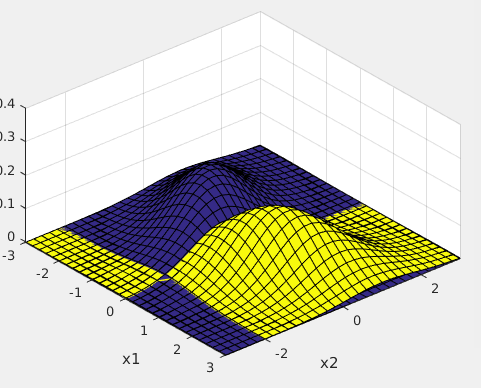
\includegraphics[scale=0.3]{Imgs/hw1-1-1.png}
\caption{Distribution of data. The distribution of class 1 is displayed in blue color and the distribution of class 2 is displayed in yellow.}
\end{subfigure}
\begin{subfigure}{0.35\textwidth}
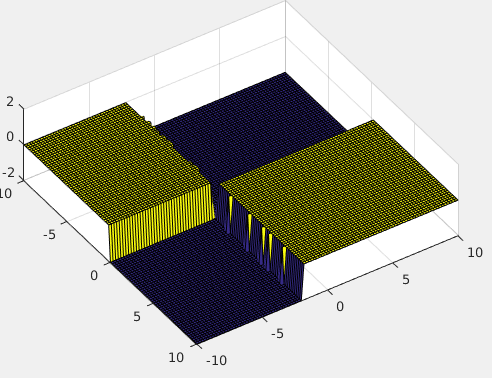
\includegraphics[scale=0.3]{Imgs/hw1-1-2.png}
\caption{Decision Boundary. The decision boundary of class 1 is displayed in blue color and the that of class 2 is displayed in yellow.}
\end{subfigure}
\caption{Bayesian Decision Boundary without considering decision costs}
\label{fig:1}
\end{figure}



\begin{center}
\line(1,0){250}
\end{center}

%%%%%%%%%%%%%%%%%%%%%%%%%%%%%%%%%%%
\item Draw the Bayes decision boundary to minimize the cost with $c_{11} = c_{22} = 0$ and
$c_{12} = 2c_{21}$ \\
The Bayesian decision boundary when considering costs of decisions turns to the form bellow:
\begin{equation}
\mathlarger{\frac{p_1(X)}{p_2(X)}} .^{>^{w_1}}_{<_{w_2}} \mathlarger{\frac{(c_{12} - c_{22})P_2}{(c_{21} - c_{11})P_1}}
\label{eq:1-1}
\end{equation}
Figure \ref{fig:4} displays the decision boundary in this case.


\begin{figure}[h]
\centering
\begin{subfigure}{0.4\textwidth}
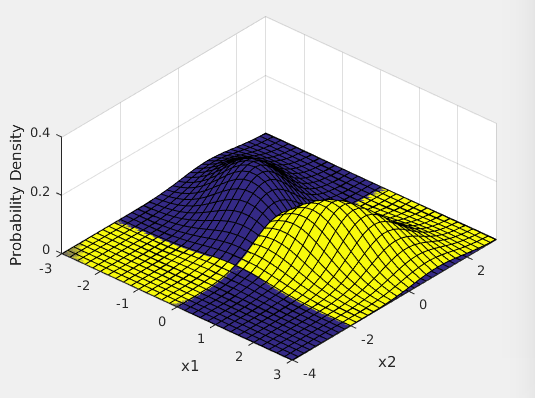
\includegraphics[scale=0.3]{Imgs/1-2-1.png}
\caption{Distribution of data. The distribution of class 1 is displayed in yellow color and the distribution of class 2 is displayed in blue.}
\end{subfigure}
\begin{subfigure}{0.4\textwidth}
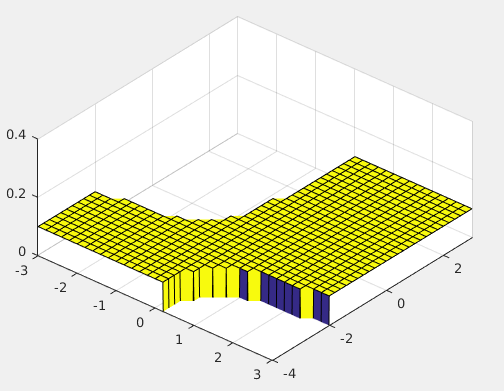
\includegraphics[scale=0.3]{Imgs/1-2-2.png}
\caption{Decision Boundary. The decision boundary of class 1 is displayed in yellow color and the that of class 2 is displayed in blue.}
\end{subfigure}
\caption{Bayesian Decision Boundary considering decision costs $c_{11} = c_{22} = 0$ and $c_12 = 2c_{21}$}
\label{fig:1-2}
\end{figure}

\begin{center}
\line(1,0){250}
\end{center}

%%%%%%%%%%%%%%%%%%%%%%%%%%%%%%%%%%%
\item Assume that $c_{11} = c_{22} = 0$ and $c_{12} = c_{21}$ :
\begin{enumerate}

\item Plot the operating characteristics.

As equation \eqref{eq:1-1} yields, with $c_{11} = c_{22} = 0$ and $c_{12} = c_{21}$ the decision boundary is not different from that of section 1. So the figure \ref{fig:1} is displaying the required decision boundary

\begin{center}
\line(1,0){250}
\end{center}

%%%%%%%%%%%%%%%%%%%%%%%%%%%%%%%%%%%
\item Find the total error when Neyman-Pearson test is performed with $\epsilon_1 = 0.05$ \\

We should estimate $\mu$ such that the following function $r$ be minimized.
\begin{equation}
r = \mu(\epsilon_1 - 0.05) + \epsilon_2
\end{equation}
After finding appropriate $\mu$, the decision boundary is derivable from:
\begin{equation}
\mathlarger{\frac{p_1(X)}{p_2(X)}} .\gl \mu
\end{equation}
To find such $\mu$ an script will iterate on following equation to reach the best fitting value.
\begin{equation}
\epsilon_1 = \int^{\infty}_\mu p_h(h|W-1) dh = 0.05
\end{equation}

The $\mu = 1.0795e-78$ is the best value estimated with $\epsilon_1 = 0.051$ error rate. Figure \ref{fig:1-3} illustrates the resulted decision boundary.

\begin{figure}[h]
\centering
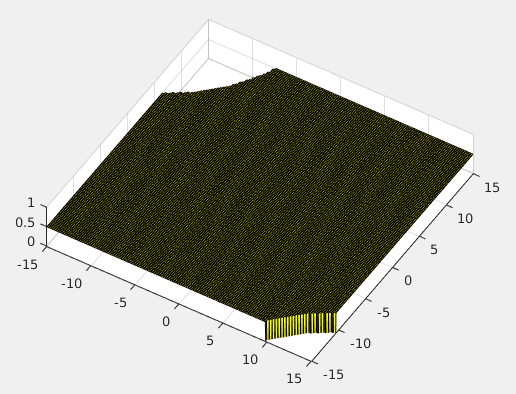
\includegraphics[scale=0.4]{Imgs/1-3-1.png}
\caption{Decision boundary resulted from Neyman-Pearson test with $\epsilon_1 = 0.05$}
\label{fig:1-3}

\end{figure}

\begin{center}
\line(1,0){250}
\end{center}

%%%%%%%%%%%%%%%%%%%%%%%%%%%%%%%%%%%
\item Find the threshold value and total error for the minimax test.

\begin{center}
\line(1,0){250}
\end{center}

%%%%%%%%%%%%%%%%%%%%%%%%%%%%%%%%%%%
\item Plot the error-reject curve.

\end{enumerate} 
\end{enumerate}


\begin{center}
\line(1,0){450}
\end{center}



%%%%%%%%%%%%%%%%%%%%%%%%%%%%%%%%%%%%%%%%%%%%%%%%%%%%%%%%%%%%%%%%%%%%%%%%%%%%%%%%%%%%%%%%%

\section{Problem 2}
Two normal distribution are characterized by: 
\begin{align*}
&P_1 = P_2 = 0.5 \\
&M_1 = \left[ \begin{matrix}
1 \\ 
0 
\end{matrix} 
\right] \> \> \> \>
\Sigma_1 = \left[
\begin{matrix}
4 & -3 \\
-3 & 4
\end{matrix}
\right] \\
&M_2 = \left[ \begin{matrix}
-1 \\ 
0 
\end{matrix} 
\right] \> \> \> \>
\Sigma_2 = \left[
\begin{matrix}
4 & 3 \\
3 & 4
\end{matrix}
\right]
\end{align*}
\begin{enumerate}
\item Find the linear discriminant function which maximize the Fisher criterion and
minimize the error by adjusting the threshold.\\
\begin{align*}
&f = \mathlarger{\frac{(\mu_1 - \mu_2)^2}{\sigma_1^2 + \sigma_2^2}} \rightarrow \frac{\partial f}{\partial \sigma_1^2} =  \frac{\partial f}{\partial \sigma_2^2} = \mathlarger{\frac{-(\mu_1 - \mu_2)^2}{(\sigma_1^2 + \sigma_2^2)^2}} \\
&\rightarrow s = \mathlarger{\mathlarger{\frac{\frac{\partial f}{\partial \sigma_1^2}}{\frac{\partial f}{\partial \sigma_1^2} + \frac{\partial f}{\partial \sigma_2^2}}}} = 0.5\\
&\rightarrow V = [0.5 \Sigma_1 + 0.5 \Sigma_2]^-1 (\mu_1 - \mu_2) = \left[\begin{matrix}
4 & 0\\
0 & 4
\end{matrix}
\right]^-1 \left[ \begin{matrix}
-2 \\
0
\end{matrix} \right] = \frac{1}{16} \left[ \begin{matrix}
4 & 0 \\
0 & 4
\end{matrix} \right] \left[ \begin{matrix}
-2 \\
0
\end{matrix} \right] \\ 
&\rightarrow V = \left[ \begin{matrix}
-0.5\\0
\end{matrix}\right] \numberthis \label{eq:1}
\end{align*}
Equation \eqref{eq:1} illustrates the best mapping vector $V$ to project distribution over, therefore the LDA will be in the form of $V^t x \geq \alpha$, in which $\alpha$ should be find from equation \eqref{eq:2}.
\begin{equation}
\frac{\partial f}{\partial \mu_1} + \frac{\partial f}{\partial \mu_2} = 0
\label{eq:2}
\end{equation}
which results:
\begin{align*}
&\frac{2\mu_1 - 2\mu_2}{\sigma_1^2 + \sigma_2^2} + \frac{- 2\mu_1 + 2\mu_2}{\sigma_1^2 + \sigma_2^2} = 0 \rightarrow 0 = 0
\end{align*}
Therefore, the best $\alpha$ is not derivable analytical. In order to estimate the best $\alpha$ a MATLAB script using bootstrapping has been written by me, which is appended to the homework submission zip file. The bootstrapping process, iterates 1000 number of times in each iteration generating 1000 multivariate random variables regarding given means and variances for each class. We attempt to estimate best $\alpha$ in each iteration using grid search in the range of $[-4,4]$ with step length 0.01. To measure the accuracy of chosen $\alpha$ we use the ratio $\frac{tp + tn - fp - fn}{N}$ as the measurement function. After all iterations, the mean of all best estimated $\alpha$s is reported as the best $\alpha$. Experiments resulted the $\alpha = 0.23$ as the best value separating two classes from each other. So the LDA function is being reformed as bellow:
\begin{equation}
\left[ \begin{matrix}
-0.5 \\ 0
\end{matrix} \right]^T X \geq^{w_1} 0.23
\end{equation}
\begin{center}
\line(1,0){250}
\end{center}

\item Find the optimum linear discriminant function which minimize the probability of
error.\\
The iterative process has been coded in MATLAB and its code is attached to the submitted homework zip file. \\
The parameter $s$ has been estimated using a grid search in rage $[0, 1]$ with step length 0.01. the error probability $epsilon$ in each iteration with respect to selected $s$ has been calculated. The figure \ref{fig:2} illustrates the behaviour of error probability w.r.t. selected $s$. The best value of $s$ is in 0 or 1. 

\begin{figure}[h]
\centering
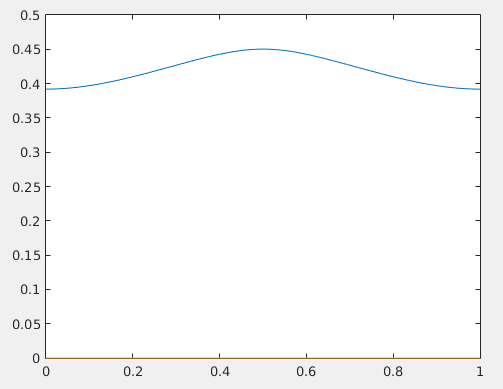
\includegraphics[scale=0.4]{Imgs/2_2_1.png}
\caption{The behaviour of error probability $\epsilon$ w.r.t. chosen $s$}
\label{fig:2}
\end{figure}

\begin{figure}[h]
\centering
\begin{subfigure}{0.4\textwidth}
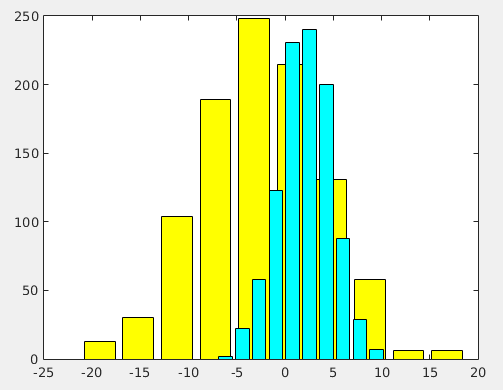
\includegraphics[scale=0.3]{Imgs/2_2_2.png}
\caption{Projected distribution of data. The projected distribution of class 1 w.r.t. mapping vector $V$ is displayed in blue color and the that of class 2 is displayed in yellow when $s = 1$ (BEST CASE).}
\end{subfigure}
\begin{subfigure}{0.4\textwidth}
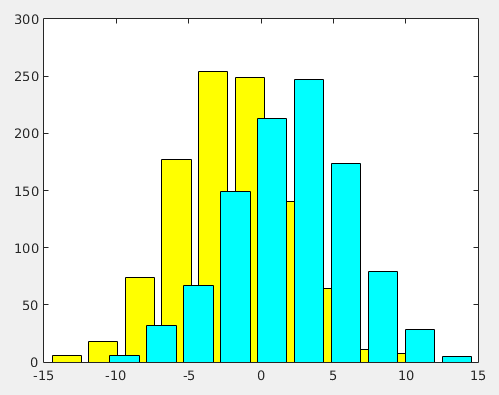
\includegraphics[scale=0.3]{Imgs/2_2_3.png}
\caption{Projected distribution of data. The projected distribution of class 1 w.r.t. mapping vector $V$ is displayed in blue color and the that of class 2 is displayed in yellow when $s = 0.5$ (WORST CASE).}
\end{subfigure}
\caption{A comparison between projected distributions over matrices $V$ w.r.t. selected $s$}
\label{fig:3}
\end{figure}


To through a light over reality, the projection of data in two cases of $s = 0.5$ and $s = 1$ has been displayed in the figure \ref{fig:3}, respectively the worst- and the best-case. As its obviously clear, the separation of classes is more suitable in case $s = 1$ rather than $s = 0.5$, hence the lower error probability will be gained when $s = 1$.



\end{enumerate}

\begin{center}
\line(1,0){450}
\end{center}

%%%%%%%%%%%%%%%%%%%%%%%%%%%%%%%%%%%%%%%%%%%%%%%%%%%%%%%%%%%%%%%%%%%%%%%%%%%%%%%%%%%%%%%%
\section{Problem 3}
We consider a classification problem in dimension $d=2$, with $k=3$ classes where:
$p ( x | w_i ) \propto N ( \mu_i , \Sigma_i ), i = 1 , 2 , 3 , $ with:
\begin{align*}
\mu_1 = \left[ \begin{matrix}
0 \\ 2
\end{matrix} \right] ,
\mu_2 = \left[ \begin{matrix}
3 \\ 1
\end{matrix} \right] ,
\mu_3 = \left[ \begin{matrix}
1 \\ 0
\end{matrix} \right] ,
\Sigma_i = \Sigma = \left[ \begin{matrix}
1 & 0 \\
0 & \frac{1}{3}
\end{matrix} \right]
\end{align*}
\begin{enumerate}
\item Calculate the discriminant function $g_i(x)$ for each class. \\
Generating a discriminant function between all pairs of classes can be a good solution. Assuming $P(W_1)=P(W_2)=P(W_3)$, the Bayes classifier is a good choice:
\begin{align*}
d_{ij}: \mathlarger{\frac{P(X|W_i)}{P(X|W_j)}}.^{>^{W_i}}_{<_{W_j}} 1
\end{align*}
Defining such classifiers, the feature function $g_i(X)$ can be defined as :
\begin{align*}
&g_1(X) = \Pi_{j=2,3}sgn(\frac{P(X|W_1)}{P(X|W_j)} - 1) \\
&g_2(X) = \Pi_{j=2,3}sgn(\frac{P(X|W_2)}{P(X|W_j)} - 1) \\
&g_3(X) = \Pi_{j=2,3}sgn(\frac{P(X|W_3)}{P(X|W_j)} - 1) \\
\end{align*}
In which the positive value of each function $g_i(X)$ indicates that $X$ belongs to $W_i$ and vice versa. 

\begin{center}
\line(1,0){250}
\end{center}

%%%%%%%%%%%%%%%%%%%%%%%%%%%%%%%%%%%
\item Express your discriminant functions in the form of linear discriminant functions. \\
The $d_{ij}$s could be expressed as linear functions as perpendicular bisectors of linking line between the center points of each class:
\begin{align*}
&d_{12} = X_2 + 3X_1 + 3 \\
&d_{13} = X_2 + \frac{1}{2}X_1 - \frac{3}{4} \\
&d_{23} = X_2 + 2X_1 - \frac{9}{2} \\
\end{align*}
Defining $d_{ij}(X) = -d_{ji}(X)$, the vector $X$ belongs to class $W_i$ iff $ \forall j \neq i , d_{ij}(X) > 0 $

\begin{center}
\line(1,0){250}
\end{center}

%%%%%%%%%%%%%%%%%%%%%%%%%%%%%%%%%%%
\item Determine and plot the decision boundaries.
Figure \ref{fig:3-1} displays the distribution of data given mean vectors and covariance matrices.
\begin{figure}[h]
\centering
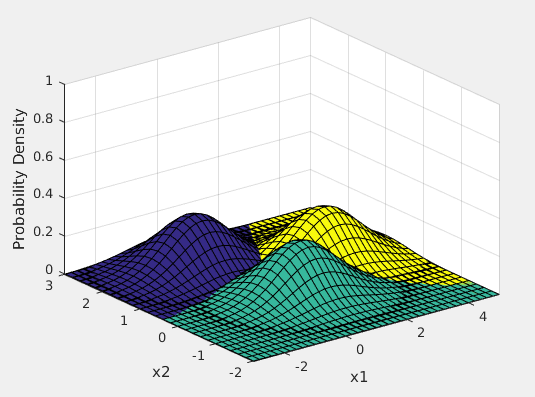
\includegraphics[scale=0.5]{Imgs/3-1.png}
\caption{Data distribution w.r.t. means and covariance matrices}
\label{fig:3-1}
\end{figure}

Figure \ref{fig:3-2} displays the data distribution boundary and deriven boundaries using two-class discriminant functions defined in section 2 of this problem.


\begin{figure}[H]
\centering
\begin{subfigure}{0.4\textwidth}
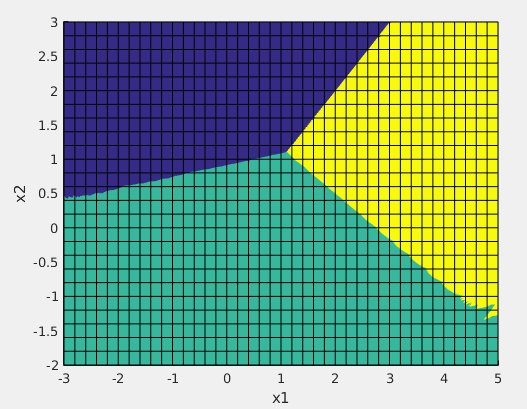
\includegraphics[scale=0.3]{Imgs/3-2.png}
\caption{Projected distribution of data on $X1-X2$ coordinates}
\end{subfigure}
\begin{subfigure}{0.4\textwidth}
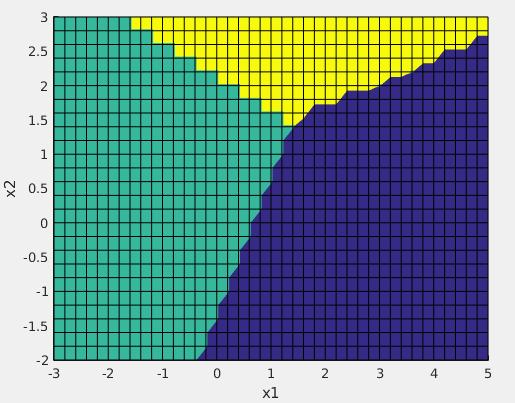
\includegraphics[scale=0.3]{Imgs/3-3.png}
\caption{Boundaries generated by discriminant functions}
\end{subfigure}
\caption{A comparison between projected distributions over matrices $V$ w.r.t. selected $s$}
\label{fig:3}
\end{figure}


\begin{center}
\line(1,0){450}
\end{center}

%%%%%%%%%%%%%%%%%%%%%%%%%%%%%%%%%%%%%%%%%%%%%%%%%%%%%%%%%%%%%%5%%%%%%%%%%%%%%%%%%%%%%%%%%%%%%%%%%%
\section{Problem 4}





\begin{center}
\line(1,0){450}
\end{center}

%%%%%%%%%%%%%%%%%%%%%%%%%%%%%%%%%%%%%%%%%%%%%%%%%%%%%%%%%%%%%%5%%%%%%%%%%%%%%%%%%%%%%%%%%%%%%%%%%%


\end{enumerate}















\bibliographystyle{plain}
\bibliography{biblist}

\end{document}